\chapter{绪论}

\section{课题来源}
红外目标检测是指用红外探测器检测目标与背景之间的红外辐射差异后,对目标进行检测的过程。虽然可见光图像具有图像分辨率高、目标细节完整的特点,但是与红外图像相比容易受到光线变化的影响,大大增加了识别目标的难度。在一些特殊的天气条件下尤其如此,例如下雨天、夜间、有雾天和缺乏可见光源的天气,视距和能见度很低,并且捕获的图像无法正常使用。红外成像技术的特点是工作距离远、抗干扰能力强、测量精度高、受天气影响较小。日夜工作和强大的烟雾穿透能力强使得红外目标检测的市场需求也在不断增加,红外目标检测不仅仅用于军事领域,在工业、安防、交通等民用领域也有广泛的应用,比如红外技术可以应用在无人机上进行全天候的目标检测;在工业界,设备有没有被严重触碰或损坏也可以应用红外技术。尤其是今年疫情期间,红外技术广泛应用于火车站、机场等人流密集的地方,能够实现实时检测体温,避免人工测量体温而造成的拥堵。

本课题主要研究红外图像中的无人机检测算法。本课题来源于哈尔滨海邻科信息技术有限公司“警用人工智能技术合作”。目前,无人机市场发展迅速,为社会带来便利。国外机场无人机干扰航班事件频发,各地无人机“黑航”事件频发。这种现象也受到了部队内外的广泛关注,给机场安全、反恐维稳和国家边境带来了相当大的压力,迫切需要通过对无人机的探测来对无人机施行监控和预警。使用声音、无线电和雷达探测的技术更为常见,但这些技术通常需要昂贵的设备和严格的配置。基于机器视觉的方法具有成本低、配置简单的优点。随着深度学习技术的发展,逐渐应用于各种目标的识别和检测,但是无人机往往在低空飞行,并且还会受到光线和遮挡等因素的影响。检测场景非常复杂,而小尺寸和高速度一直是目标检测的难题。相关监管部门需要利用相关检测网络及时发现管制区域内的非法无人机,以保障人身安全和财产安全。因此,本课题的目的是研究和设计无人机检测算法,以实现快速高效的红外无人机检测。

\section{研究背景与意义}
计算机视觉技术是一种让计算机从给定的图像或视频中获取相关信息并进行“感知”的技术,是人类视觉感知的扩展。半导体行业促进了硬件水平的提高,也带动了机器视觉的发展,使其在人工智能领域得到广泛应用。

随着各方面技术的成熟,研究人员在不断提高红外探测系统的性能。红外探测技术广泛应用于军事领域,如红外预警、水下搜索和红外导航中,还应用于医疗损伤、细胞诊断、工业探伤等民用领域,在军事和包括医疗在内的民用领域取得突出成就。
自1960年代初以来,红外热成像已经开始用于医学\cite{ring1975thermography}。早期的成像系统很大,显示和测量温度的设施非常有限
。在 1970 年代,热像图的计算机图像处理投入使用,增加了对图像进行定量和存档的可能性。如在疾病诊断和预防领域,大多数风湿性疾病的共同因素是关节炎。 辐射测量和热成像已被证明可以指示和测量由局部炎症引起的发热。 在类风湿性关节炎、幼年型关节炎、骨关节病、痛风和强直性脊柱炎中,受累关节的热量分布异常。 实验数据表明,温度变化反映了关节的炎症状态,这一结论可用于衡量口服、全身和局部药物治疗以及手术(即滑膜切除术)的治疗效果。

在计算机视觉领域中,当前主流的探测系统可分为3类:可见光探测、红外成像探测和雷达探测系统,基于红外探测系统的红外弱小目标检测一直都是一个重要的课题和研究热点。红外探测系统主要对对目标的温度与本身的材料特性敏感,而与环境等因素相关性较小,使得其在3类探测系统中脱颖而出,具有一系列优势:
(1)不受光照的影响,可以全天时工作;
(2)由于其不发射电磁波,因此是非主动的探测方法;
(3)穿透能力强,可以避免灰尘、云层和烟雾等的遮挡,可以更好地识别虚假的伪装目标。以上优势也使其成为传统可见光探测系统与雷达探测系统的有效补充或替代。

实时检测红外目标,高检出率、低误报率是实际应用中重要的要求。一般情况下,待检测目标与检测器之间的距离较长,因此,红外目标在整个红外图像中占据的区域非常小。它们通常小于 100 像素,背景复杂、易变且难以检测。具体表现如下:

(1)红外目标的特点:弱小红外目标缺乏颜色、纹理等属性,尺寸较小。 (通常小于 9×9 像素)大多数方法仅适用于灰度分布特征、运动属性和运动方向等特征。此外,小型红外目标的信噪比较低。并且经常被复杂而动态的背景所掩盖,还会受到云层和海浪的干扰。

(2) 红外背景的特点:背景相似,分布连续。目标通常在云和波浪中。场景复杂多变。复杂红外图像的背景特征有些不均匀,并且相对灰度比目标区域低。

(3) 红外目标检测中的困难: 1) 目标的可用特征较少。因为目标很小,所以总辐射能量小于背景辐射能量。图像中的灰度分布是可变的,很难使用统一的数学模型来描述,而且它缺乏传统可见光目标的纹理、形状和其他结构信息。传统可见光检测方法不能用于检测小而弱的红外目标,或是一般性能较差。 2)图像的信噪比低。由于成像距离远,小目标难以和杂波和噪声区分开,容易被淹没在云层和海浪中,使得检测算法容易受到干扰。 3)检测精度往往不高。在实际情况和使用中,目标的运动方向和速度具有很强的机动性。这使得提高机动目标的检测精度成为学术界致力于解决的问题。4)成像环境复杂。在特种成像方面,成像过程往往伴随着烟雾和海浪。这导致对不同检测算法的鲁棒性提出更高的要求。 5)实时性较差。检测效果通常与计算量成近似反比。检测效果好的算法往往需要大量的计算。因为建模体积大、硬件处理能力不足,常常导致实时性能不佳。6)很少有公开数据集。红外目标检测主要用于军事领域,具有一定的保密性。可供研究人员公开使用的红外数据集很少,这在一定程度上限制了红外目标检测算法的发展。本课题检测的目标图像如图\ref{uav}所示。

\begin{figure}[htbp]
    \centering
    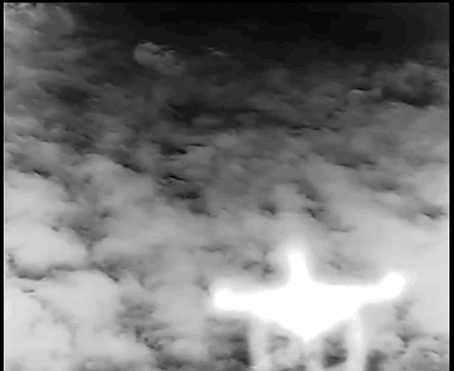
\includegraphics[width = 0.8\textwidth]{无人机目标示例.png}
    \caption{无人机目标示意图}
    \label{uav}
\end{figure}

综上所述,红外图像的无人机目标检测应用广泛,研究价值很大。本文基于深度学习算法,针对红外无人机目标进行研究,针对红外图像无人机目标检测的特点,从数据增强、网络结构改进、网络轻量化、嵌入式实现这四个方面展开研究。

\section{国内外研究发展现状}
目标检测算法一般包括分类和定位两个子任务,常用于检测图像中某些已知类别的对象。本节主要从传统的目标检测算法、基于深度学习的两阶段目标检测算法、基于深度学习的单阶段目标检测算法以及针对红外图像的目标检测算法4个方面来介绍本文研究领域目标检测算法的研究现状\cite{尹宏鹏2016基于视觉的目标检测与跟踪综述}。

\subsection{传统的目标检测算法}
如图\ref{ct}所示,传统的目标检测算法流程是首先通过某种算法得到选定的待检测区域,对该区域经过特征提取,最后输入分类器进行分类后得到检测结果。

\begin{figure}[htbp]
    \centering
    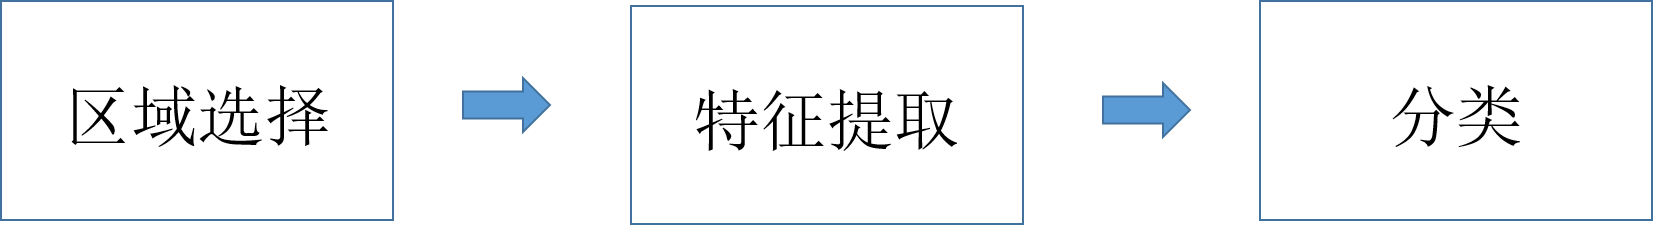
\includegraphics[width = 0.6\textwidth]{传统目标检测.png}
    \caption{传统目标检测流程}
    \label{ct}
\end{figure}

传统的目标检测算法在进行计算时,对于初始区域的选择是使用遍历的方式搜索整个图像的不同比例纵横比的滑动窗口,得出候选区域,即某个可能包含目标的区域\cite{胡伏原2020基于卷积神经网络的目标检测算法综述,kira1992feature}。这种暴力穷举法的特点是时间复杂度很高,而且会产生大量的重复窗口,不仅影响后续的特征提取的准确性,而且会拖慢整个算法的运行时间。后来研究人员设计了效率更高的区域选择算法,比如有选择性搜索算法(Selective Search)\cite{uijlings2013selective}以及Edge Boxes算法\cite{zitnick2014edge}等。选择性搜索算法首先将原始图像划分为多个尺寸较小区域,然后根据计算出的某两个区域之间的相似度和这两个区域的大小依次组合相邻的小区域,反复执行上述过程,直到在整幅图像内组合成一个大区域。Edge Boxes算法则是充分利用若干个edge box相互之间潜在的相似性,根据权重的值来确定某个box中包含的轮廓的数量或与该box的边界产生重叠的轮廓的数量,之后根据上述统计信息对每个box进行打分和评估,确定出候选box。之后的第二步是从候选区域中通过特定的特征提取算法提取特定长度的特征向量,以获得该区域的语义信息,做出对目标分类的预测。一般情况下,包括在目标检测领域中,传统机器学习算法会选择向机器学习模型中输入工艺特征。然而,由于物体的形状和尺寸多变、光照会随时间和天气不断变化、背景的多样性,设计一种鲁棒的特征提取算法往往比较困难,而提取特征模块的性能好坏直接影响到后续的分类模块的准确性。在特征提取的阶段,HOG函数\cite{he1990texture}和SIFT函数\cite{lowe1999object}是较为常用的特征表达函数。HOG算法首先会将图像分割成一些小的连通区域(细胞单元),之后在每个单元处对每个像素点的梯度直方图进行采样,或是对单元边缘区域的梯度直方图进行采集,HOG算法将用这种方式获取的直方图称作该单元的特征。与其他的特征描述方法相比,HOG有很多优点。首先,由于HOG是在图像的局部方格单元上操作,所以它对图像几何的和光学的形变都能保持很好的不变性,这两种形变只会出现在更大的空间领域上。其次,在粗的空域抽样、精细的方向抽样以及较强的局部光学归一化等条件下,只要行人大体上能够保持直立的姿势,可以容许行人有一些细微的肢体动作,这些细微的动作可以被忽略而不影响检测效果。
因此HOG特征比较适合用于图像中的人体检测任务。SIFT算法的处理方法是首先计算出输入图像的DoG尺度空间,之后在该DoG空间中求出极值点,然后调整尺度空间DoG函数,拟合出近似的DoG函数,以准确找到关键点,并去除不稳定的关键点。然后计算剩余关键点的主要方向用以创建 SIFT 描述子。SIFT函数的特点是具有尺度不变性和旋转不变性,此外还具备适应复杂光照背景变化的能力,因此在传统目标检测算法中得到广泛应用。

在完成对图像特征的提取之后,算法将使用分类器对待测目标进行分类。
分类器相关算法主要有Adaboost\cite{freund1997decision} 算法等,而经典的分类器主要有SVM\cite{cortes1995support}分类器等。
常用于对分类器进行优化的AdaBoost算法属于一种常见的Boosting算法。
Boosting, 也称为增强学习或提升法,是⼀种重要的集成学习技术,能够将预测精度仅⽐随机猜度略⾼的弱学习器增强为预测精度⾼的
强学习器,这在直接构造强学习器⾮常困难的情况下,为学习算法的设计提供了⼀种有效的新思路和新⽅法。其中最为成功的应⽤就是AdaBoost算法。
AdaBoost是英⽂"Adaptive Boosting"(⾃适应增强)的缩写,它的⾃适应在于:前⼀个基本分类器被错误分类的样本的权值会增
⼤,⽽正确分类的样本的权值会减⼩,并再次⽤来训练下⼀个基本分类器。同时,在每⼀轮迭代中,加⼊⼀个新的弱分类器,直到达到某个
预定的⾜够⼩的错误率或达到预先指定的最⼤迭代次数才确定最终的强分类器。
Adaboost算法的流程可以简述为三个步骤:

 (1)⾸先,初始化训练数据的权值分布。假设有$N$个训练样本数据,则每⼀个训练样本最开始时,都被赋予相同的权值。

 (2)然后,训练弱分类器。具体训练过程是:如果某个训练样本点,被弱分类器准确地分类,那么在构造下⼀个训练集中,它对应
的权值要减⼩;相反,如果某个训练样本点被错误分类,那么它的权值就应该增⼤。权值更新过的样本集被⽤于训练下⼀个分类器,整个训
练过程如此迭代地进⾏下去。

 (3)最后,将各个训练得到的弱分类器组合成⼀个强分类器。各个弱分类器的训练过程结束后,加⼤分类误差率⼩的弱分类器的权重,使
其在最终的分类函数中起着较⼤的决定作⽤,⽽降低分类误差率⼤的弱分类器的权重,使其在最终的分类函数中起着较⼩的决定作⽤。误差率低的弱分类器在最终分类器中占的权重较⼤,否则较⼩。

支持向量机(support vector machines, SVM)是一种二分类模型,它的基本模型是定义在特征空间上的间隔最大的线性分类器,间隔最大使它有别于感知机;支持向量机还包括核技巧,这使它成为实质上的非线性分类器。支持向量机的学习策略就是间隔最大化,可形式化为一个求解凸二次规划的问题,也等价于正则化的合页损失函数的最小化问题。支持向量机的学习算法就是求解凸二次规划的最优化算法。

传统的机器学习算法对于目标检测问题能取得一定的检测效果,但是对于复杂任务还是存在性能瓶颈。分析其算法原理可以发现传统的目标检测算法都存在两个问题:

(1)算法的复杂度高,在整体流程较为冗长、步骤较多的同时,各个部分单独的时间复杂度也较高,因此整体效率往往较低。具体到区域选择算法中,虽然区域选择算法从原始的滑动窗口算法到选择性搜索算法已经有了较大的效率提升,但是仍然存在选择过程没有针对性的固有问题,结果中仍然会保留相当数量的多余窗口,会影响到后续的分类模块的检测精度和速度。

(2)手工设计的特征往往带有一定的特殊性,因此对于目标检测任务的多样性往往难以匹配足够的泛化能力,在背景和目标尺度等条件变化较大时,手工设计的特征难以适应这些变化,往往无法准确地获取目标的语义信息,因此检测的精度会产生较大波动,总体精度不高。

因此区别于传统的目标检测算法的流程冗长和可学习特征量不足等问题,深度卷积神经网络能较好地部署端到端的系统算法,能从整个流程上优化算法的运行效率。此外,深度卷积神经网络能容纳更多的模块和参数,也就是能拟合更加复杂的目标函数,在充分训练之后,深度神经网络对输入信息的捕捉和表达能力更强。并且随着相关研究的持续进行,深度卷积神经网络可以将网络分成各类具有特殊功能的模块,比如可以将位置信息和语义分类信息通过不同的网络层进行提取和增强。正是因为基于深度学习的目标检测算法相对于传统机器学习检测方法有很多显著的性能优势,同时随着计算机计算能力的快速发展,基于深度学习的目标检测算法成为了重点研究领域,研究人员不断设计各种新算法,不断在目标检测任务中取得更好的性能。

\subsection{基于深度学习的两阶段目标检测算法}
两阶段目标检测算法也称为基于候选框的目标检测算法。这种目标检测算法主要分两步进行:

(1)通过对输入图像的计算,应用特定算法得出若干候选区域。这一步骤中经常使用的算法有选择性搜索和Edge Boxes等。

(2)对候选区域应用卷积神经网络(Convolutional Neural Networks, CNN)进行推理,卷积神经网络主要用于特征的提取和得出分类结果。

2014 年,Girshick 等人开创性地提出不再使用传统的
滑动窗口+手工特征的目标检测方法,而是使用选择性搜索+卷积神经网络进行代替。经过研究后提出了 R-CNN 模型框架\cite{girshick2014rich},经过实验,证明了卷积神经网络相比于传统的 HOG
等手工特征在 PASCAL VOC 2007数据集上的目标检测性能更好,进一步说明了深度学习算法
在目标检测领域的有效性和优越性,以该算法为起点,掀起了一波研究基于深度学习的目标检测算法的风潮。如图
\ref{rcnn}所示,R-CNN算法的流程主要由 4 个步骤组成:

\begin{figure}[htbp]
    \centering
    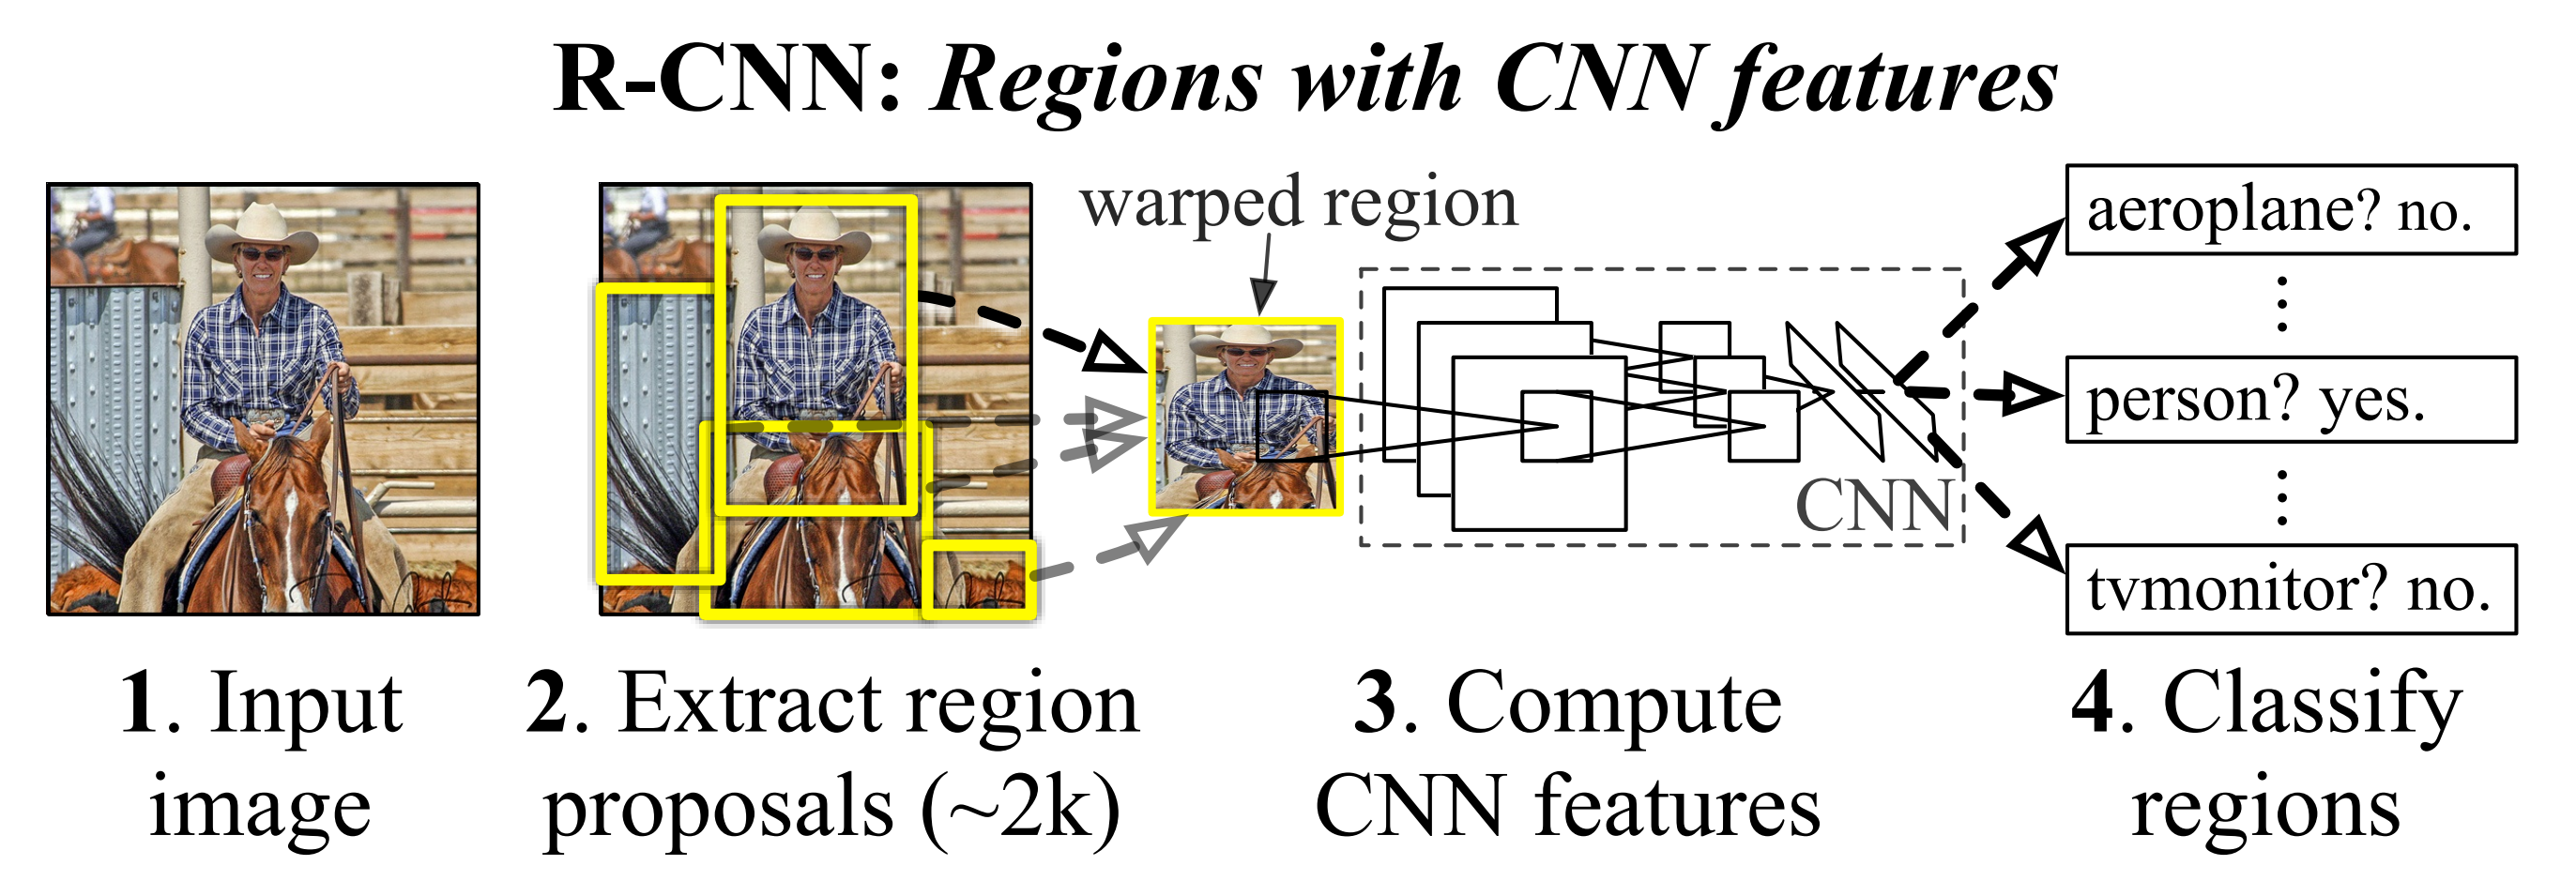
\includegraphics[width = 0.7\textwidth]{rcnn.png}
    \caption{R-CNN算法框架}
    \label{rcnn}
\end{figure}

(1)对于每张输入图片,通过选择性搜索
算法产生 $1000\thicksim2000$个候选区域,把这些区域经过缩放后调整到后续网络需要的大小。

(2)对每个候选区域分别使用卷积神经网络提取目标的特征,将提取的特征以特征向量的形式输出。

(3)在接收到前序模块输出的特征向量作为输入后,支持向量机分类器进行分类,对于每个类别分别训练各自的分类器,各个分类器之间相互独立,不共享参数。

(4)因为候选框是经过不完善的选择型搜索算法计算得出,因此需要对候选框位置进行适当修正,这一过程一般情况下使用 bounding-box 回归器。

经过分析算法原理可知,相比于传统的目标检测算法,卷积神经网络的特点是能在不同层网络捕捉到特定目标的待求尺
寸信息,并且经过计算可以生成的特征图能够充分表征目标的各种特征。R-CNN模型对 AlexNet 网
络结构进行了应用,此外还借鉴并优化了 fine-tuning方法。经过在 PASCAL VOC 2007 数据集上的实验证明,准确率可以达到 $58\%$,而使用 VGG16 网络结构的版本在 PASCAL VOC 2007 数据集上的准确率达到 $66\%$,这个结果
和传统算法相比高了约 $20\%$。

但是R-CNN算法并不完美,主要有以下3个问题:

(1)整个算法网络结构训练需要分为好几个阶段,训练时间长,步骤繁琐的同时容易产生错误。

(2)区域选择算法的效率仍然存在改进空间。选择性搜索算法会导致每张图片提取到过多的候选区域,存在较多冗余候选区域,常常增加训练耗时,大大影响算法的整体效率。并且选择性搜索算法的鲁棒性有限,很难保证在复杂背景下选择出高质量的候选框。

(3)候选区域提取算法不仅仅会产生大量冗余的候选框,这些提取到的候选框是分别进入到卷积神经网络中进行特征提取,因此除非对算法进行特别设计的并行优化,该算法无法避免地会产生大量重复的无用计算,大大降低算法的时间效率。

之后何凯明等人经过研究空间金字塔匹配(SPM)概念,特别针对 R-CNN 在
提取特征时存在重复计算等问题,提出了创新的SPP-Net\cite{purkait2017spp},有效地解决了R-CNN 对所有的候选
区域全部无选择地输入网络提取特征的问题。主要方法是对整张图片一次性地利用卷积神经网络提取特征,
并将提取到的特征通过 SPP 转变成固定长度的特征向量,之后将特征向量输入到全连接层。这样就实现了加快
R-CNN 的目标,同时还减少了算法的计算量。SPP的流程不经过原来R-CNN 中输出固定大小候选区域的处理步骤,因此也不会引起信息的丢失和引发几何失真等问题。但
SPP-Net仍然存在局限性。SPP-Net不能使用梯度反传算法(BP)对某些层的参数进行更新,
并且SPP-Net的训练仍然是多阶段过程。此后,经过研究SPP-Net 的两个局限点后,2015 年 Girshick 提
出的 Fast R-CNN\cite{girshick2015fast}算法首创性地将SPP-Net 和 R-CNN 的优点进行结合,不仅提取特征的方式改进成一次性地将整张图像输入到网
络中进行,还应用了多任务损失函数(主要是分类和回归等),最终结果是整个训练过程除
了提取候选区域以外的过程都实现了端到端优化,这一改进也大幅优化了 R-CNN 中存在的多阶段训练和
存储而消耗大量时间和存储资源的问题。该算法的创新点有:

(1)和以往的R-CNN算法不同,Fast R-CNN开创性地将分类损失函数和回归损失函数融合起来组成一种新的复合损失函数,
统一进行网络的训练。

(2)使用 softmax 取代原来的支持向量机分类器。

(2)设计使用ROI池化模块。ROI
池化层是一种相比 SPP-Net 空间金字塔池化层更简洁的池化层模块,主要作用是能将图像
应用候选框选择算法计算得出的候选框添加到最后一个卷积层输出的 特征图 上,
之后经过 ROI池化输出固定大小(一般所使用的为最大池化)。经过实验,Fast R-CNN算法在
PASCAL VOC 2007 数据集上的mAP 可以达到 $66.9\%$,虽然相比于 R-CNN 仅仅提升了 0.9
个百分点,但是Fast R-CNN的训练速度达到了R-CNN算法的 9 倍。

Fast R-CNN算法仍然存在问题。该算法的局限性主要是仍然没有拜托相对低效的区域选择算法,Fast R-CNN使用的选择性搜索或 Edge Boxes 算法主要基于相对固定的低级视觉信息,也就是无法通过数据驱动方式进行学习和进化,并
且时间效率较低。Fast R-CNN算法的主要框架如图\ref{fastr}所示。

\begin{figure}[htbp]
    \centering
    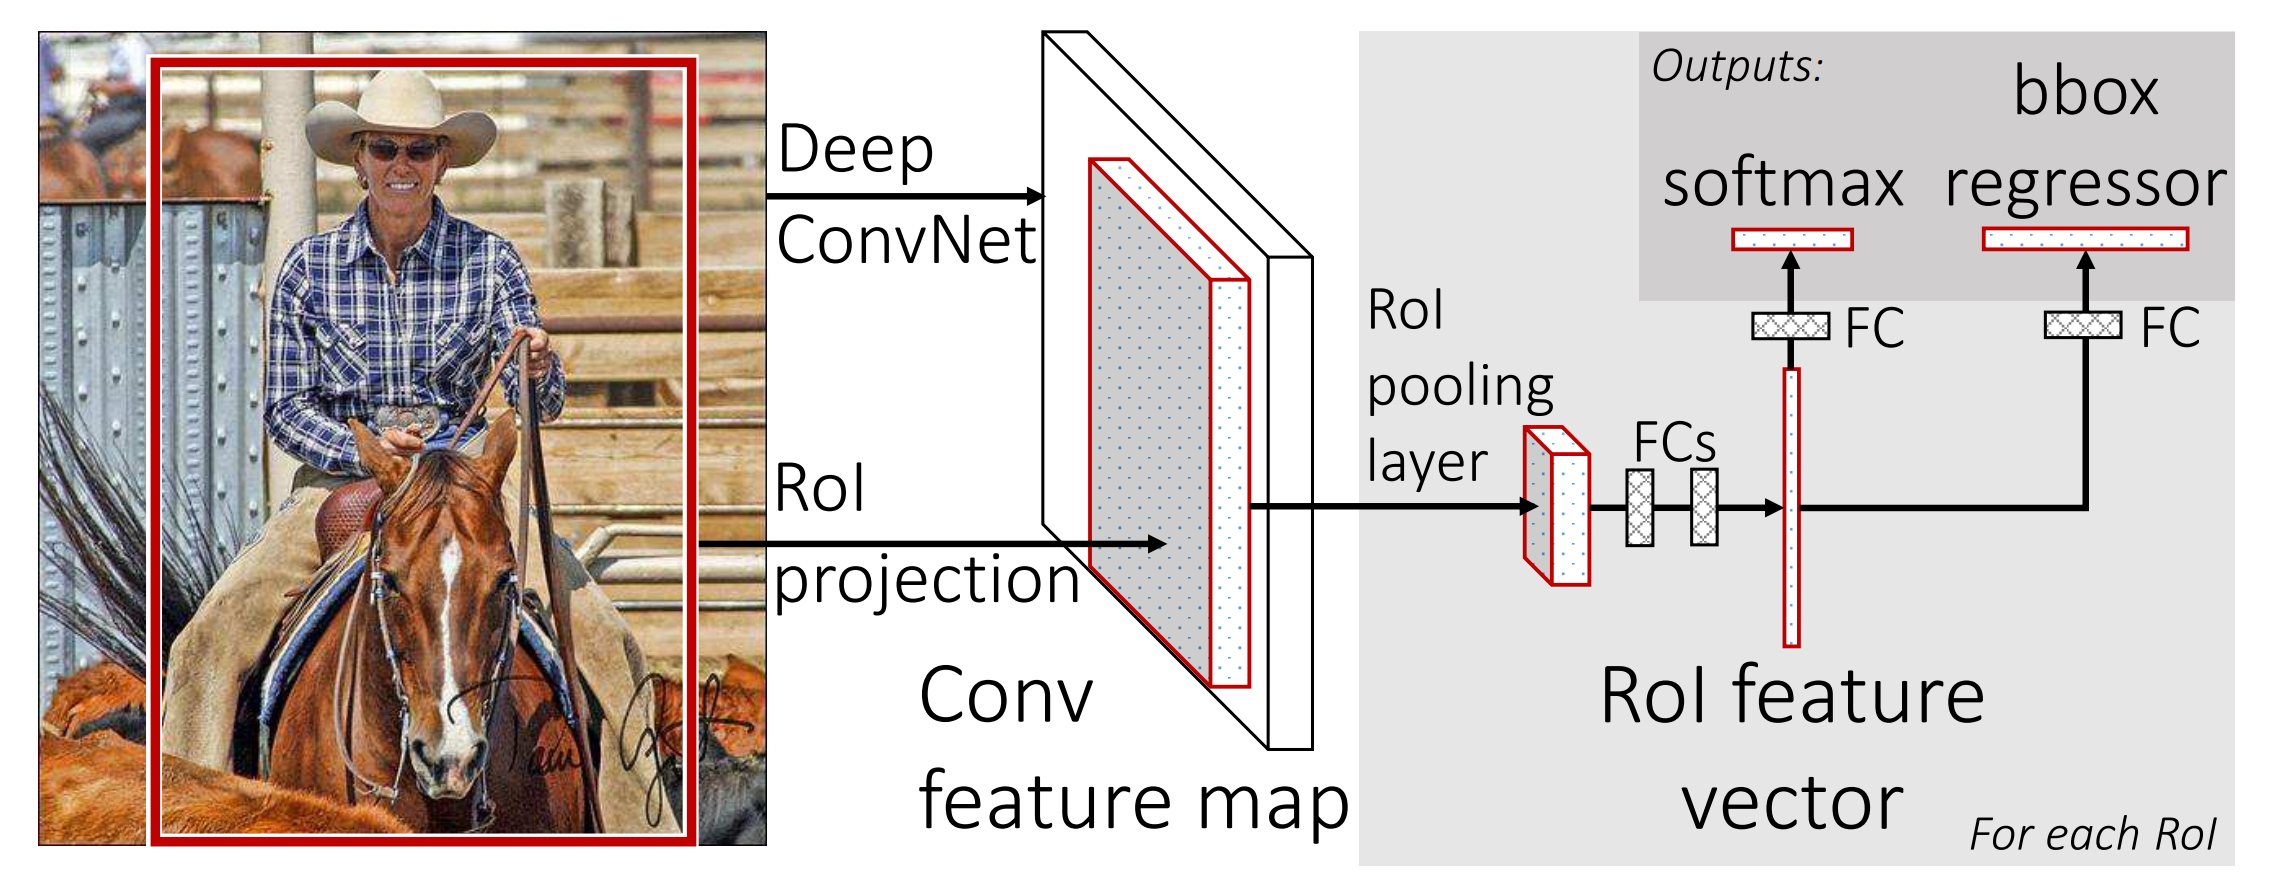
\includegraphics[width = 0.9\textwidth]{fastr.png}
    \caption{Fast R-CNN算法框架}
    \label{fastr}
\end{figure}

2016 年,Ren 等人针对 R-CNN系列算法的候选区域算法普遍存在的候选区域提取速度的问题,研究并提出了 Faster R-CNN 算法
\cite{ren2015faster},Faster R-CNN 算法的主要框架如图\ref{fasterr}所示。

\begin{figure}[htbp]
    \centering
    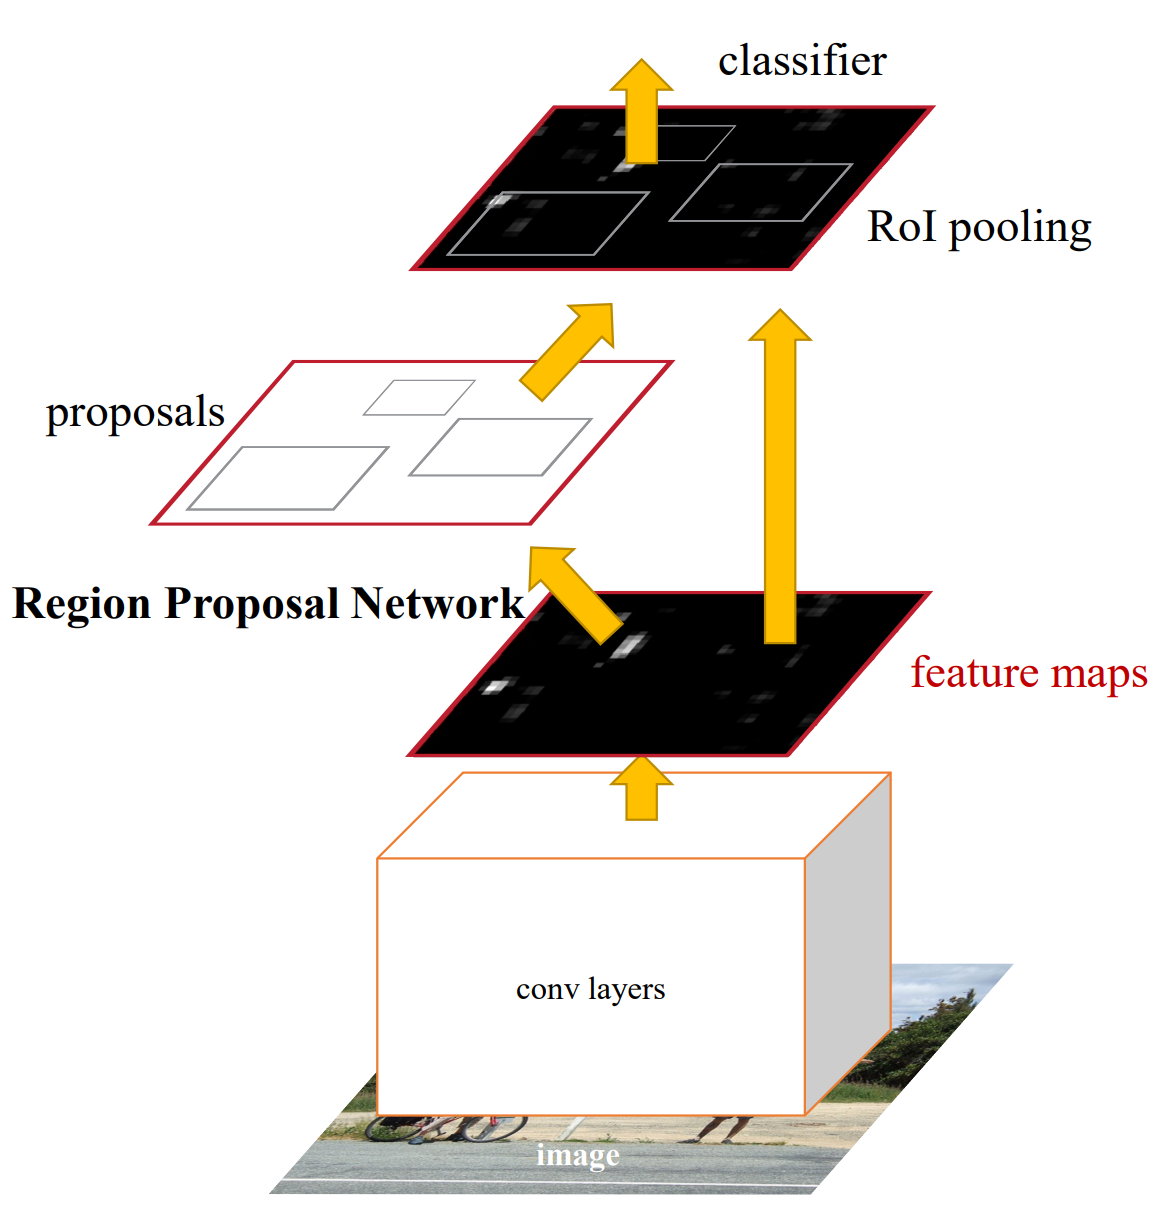
\includegraphics[width = 0.7\textwidth]{fasterr.png}
    \caption{Faster R-CNN算法框架}
    \label{fasterr}
\end{figure}

Faster R-CNN 算法的主要贡献是创新地使用 Region
Proposal Network(RPN)网络替代选择性搜索算法,由于 RPN 与检测网络主体
共享全部的卷积特征并且还有一组公共的卷积层,因此可以实现算法网络的端到端训
练。Faster R-CNN 算法的实现过程是:

(1)将输入图像输入VGG-16网络进行特征的提取。

(2)使用 RPN 生成proposals。RPN 是一种全卷积网络,能够通过 $n \times n$ 的滑动窗口在特征
图上逐点滑动,在特征图的每个位置上以窗口为中心用 9 种(三种尺度,三种长宽比)
anchor 生成 proposals,然后对每个 proposal 进行判断,判定其是否为背景,并进行初步的回归。

(3)将 RPN 得到的的输出作为输入送进Fast R-CNN,通过 ROI池化输出固定大小 特征图 后进行更为精细的分类工作,此外对检测框的位置进行进一步修正。

Faster R-CNN 的NIPS2015 版本使
用的主要框架是 RPN+Fast R-CNN 网络,整体流程跟 Fast R-CNN一样。经过实验,该算法在 PASCAL VOC 2012 数据集上的mAP 可以达到$73.2\%$,此外该算法具备比Fast R-CNN快10倍的运行速度。

Faster R-CNN 算法的局限主要集中在以 ROI 池化层为界,网络的功能较为固定,前面一部分子网络用于特征提取,后面
一部分子网络用于目标检测,并且在对候选框分类和回归任务需要分别在全卷
积网络中进行各自的计算,因此算法整体的计算量仍然很大,该算法仍然在多数情况下达不到实时检测的要求,并且对小尺寸目标的检测效果比较差。

通过研究人员的不懈努力,基于候选框的目标检测算法在 Faster R-CNN 之后仍然在不断进步,目前具
有代表性的主要有 R-FCN\cite{dai2016r}和 Mask R-CNN\cite{he2017mask}。Faster R-CNN 的问题在于虽然初步实现了网络的端到
端训练,但是整个网络以 ROI 池化层为界前面是共享全卷积网络,后面是分类网络,不能达到共享计算的效果,因此整个算
法运行的时间效率较低。而经过理论研究,算法所使用网络的backbone卷积层数越深,就能获得有意义的语义特征,进而更加有利于最终的分类任务的正确完成。但是与此同时,网络层数加深会导致目标的位置信息丢失
,最终会使得算法对待测目标的定位能力受损。

由于目标检测的任务是对图像中的待测目标进行位置和分类的求解,通过对ResNet、GoogLeNet
提出的分类网络和检测网络的平
衡问题进行研究与分析,R-FCN 提出了一种position-sensitive score mAP的概念。R-FCN 的backbone采用ResNet-101(去
掉最后一层 FC 层),将conv4层的输出作为 RPN 的输入,计算得到ROI,之后将网络
最后输出的 特征图用来计算position-sensitive score mAP,分别进行回归和分
类。经过实验证明,R-FCN可以在不损失精度的情况下获得比 Faster R-CNN大2.5 倍的运行速度。算法框架如图\ref{rfcn}所示。

\begin{figure}[htbp]
    \centering
    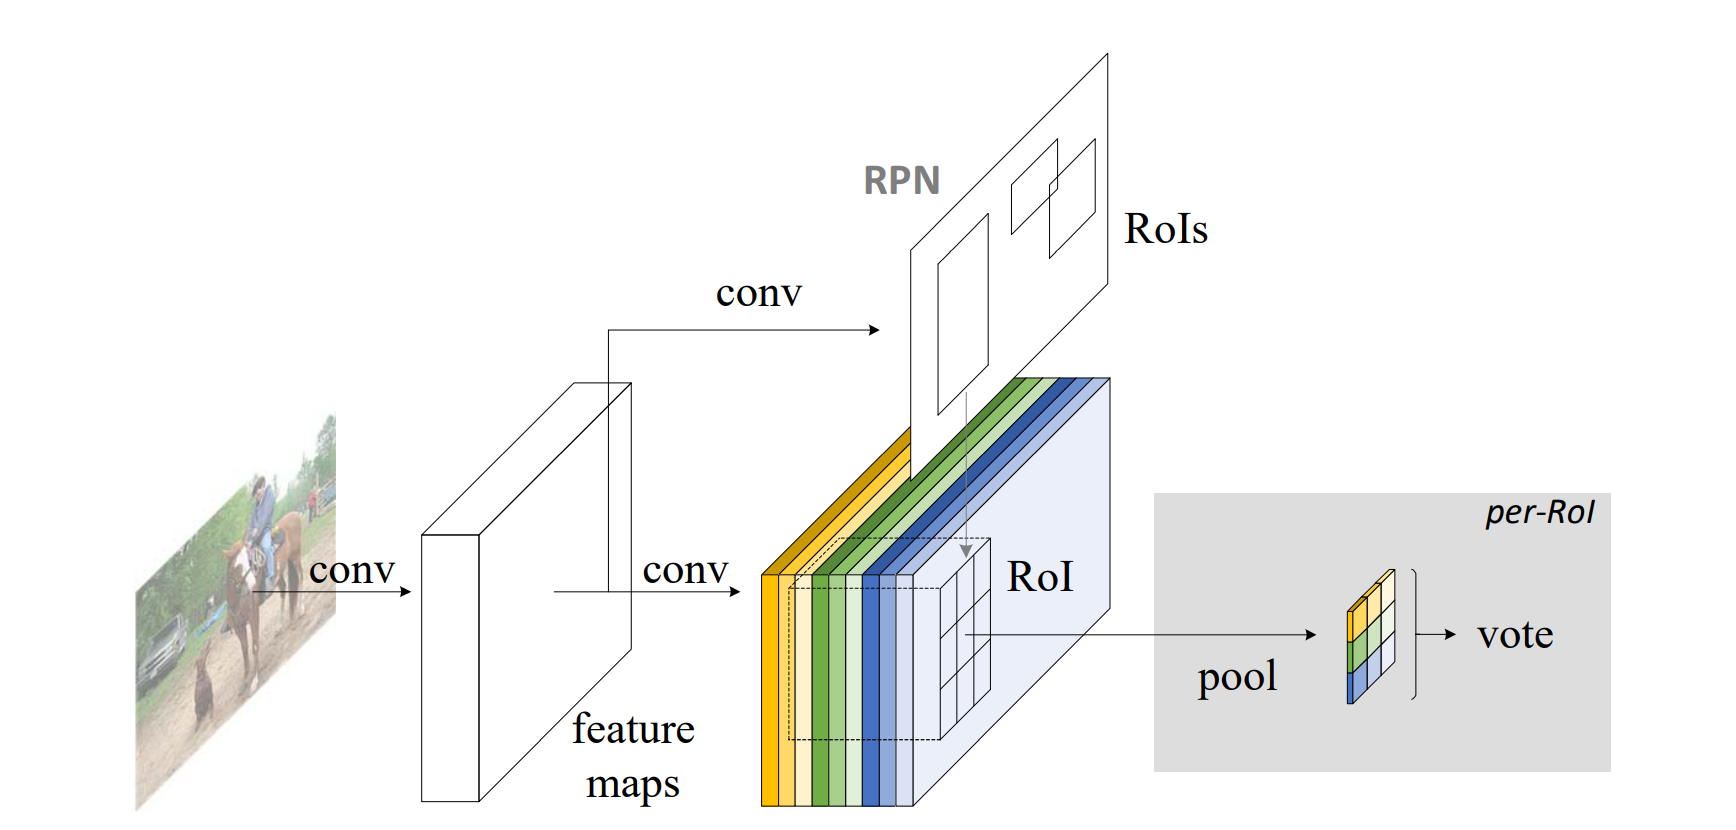
\includegraphics[width = 0.9\textwidth]{rfcn.png}
    \caption{R-FCN算法框架}
    \label{rfcn}
\end{figure}
在Faster R-CNN的基础上,Mask R-CNN添加了一个预测目标掩模的并行分支,称为mask分支,该分支的主要作用是为每个目标实例产生高质量的分割掩模,从而与原本的Faster R-CNN并行地进行目标检测和目标实例分割任务。Mask R-CNN是一个简单的、易于训练的网络,相对于Faster R-CNN只增加了少量的运算,能够以5 fps的速度运行。此外,Mask R-CNN能够较好地扩展到人体姿态估计等其他任务上。在COCO的3个挑战任务(实例分割、目标检测、人体关键点检测)中,Mask R-CNN都取得了当时的最好成绩。该算法主要的创新在于提出了ROI Align算法。该算法主要研究了目标检测中特征图上可能出现的目标的定位不是整数的问题。在ROI池化层中需要对特征图进行一定程度的缩放,该过程容易引入量化误差,虽然量化本身产生的误差较小,但是这个误差按比例映射到原图上就会被放大,从而影响算法对目标定位的精度。ROI Align算法就是用一种双线性插值的方法补充这些位置的像素点,用最大池化或者平均池化的方法取代量化,从而规避量化误差,提高算法模型对目标的定位能力,算法框架如图\ref{maskr}所示。

\begin{figure}[htbp]
    \centering
    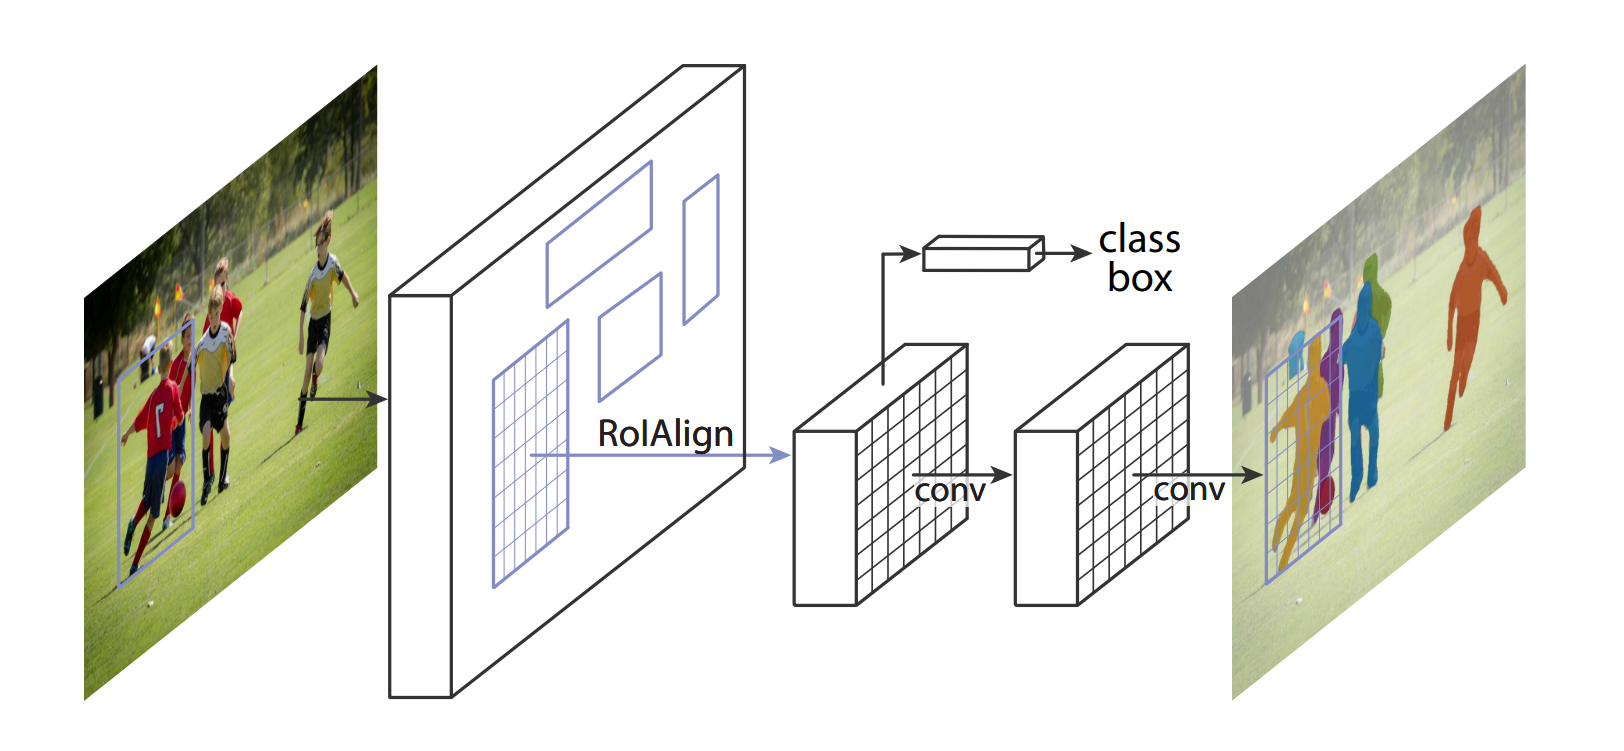
\includegraphics[width = 0.9\textwidth]{maskr.png}
    \caption{Mask R-CNN算法框架}
    \label{maskr}
\end{figure}

\subsection{基于深度学习的单阶段目标检测算法}
上文提到的两阶段目标检测算法,又称基于候选框的目标检测算法,主要特点是将整个图像的目标检测问题分割成确定区域和对待测区域进行分类两个独立的任务,因此该类型的目标检测算法往往存在速度上的瓶颈。想要从这个角度突破性地优化目标检测的推理速度,关键是将选择区域和进行分类这两个任务联合起来,方便总体优化时间的同时,能将图像中各区域间的信息联合起来,充分利用上下文之间的相关性。基于这些分析,研究人员提出了一种基于回归的目标检测算法,这种算法的显著特征是将目标检测问题转化成回归问题,对图像中的若干个位置直接进行目标检测和分类,从而达到跳过单独的区域选择阶段\cite{jiao2019survey,wu2020recent}。
2016 年 Redmon 等人提出了 YOLO(You Only Look Once)算法\cite{redmon2016you}。YOLO之前的目标检测方法,都是在不断对分类网络进行优化以提高算法的性能。相反的,作者把目标检测视为一种对目标框和类别的回归问题。该算法应用了一种简单的神经网络,对整个图像直接预测目标边框和对应的类别。由于整个的检测流程就是一个单独的网络,使得该算法端到端地优化检测的速度。YOLO框架在当时是非常快速的。基础的YOLO模型每秒可以处理45个图像,而一个较小版本的YOLO模型(Fast YOLO)速度达到了155FPS的同时,mAP也比其他的检测算法高2倍。YOLO算法与当时最好的检测算法相比,虽然会出现更多的定位错误,但是对于把背景预测成目标的错误出现频率要低很多。
YOLO 框架为图\ref{yk}所示,YOLO算法的检测网络包括24个卷积层,之后是2个全连接层。交替的$1\times1$卷积层能够起到减少前一层的特征空间的作用。YOLO算法可以在ImageNet分类任务上以一半的分辨率(输入图像分辨率是$224\times224$)对网络中的卷积层进行预训练,在预训练后通过将分辨率加倍的方式进行目标检测。
YOLO算法能够直接在输出层对目标进行位置和所属类型的回归,实现了真正意义上的单阶段检测。YOLO算法进行目标检测的主要流程是:

\begin{figure}[htbp]
    \centering
    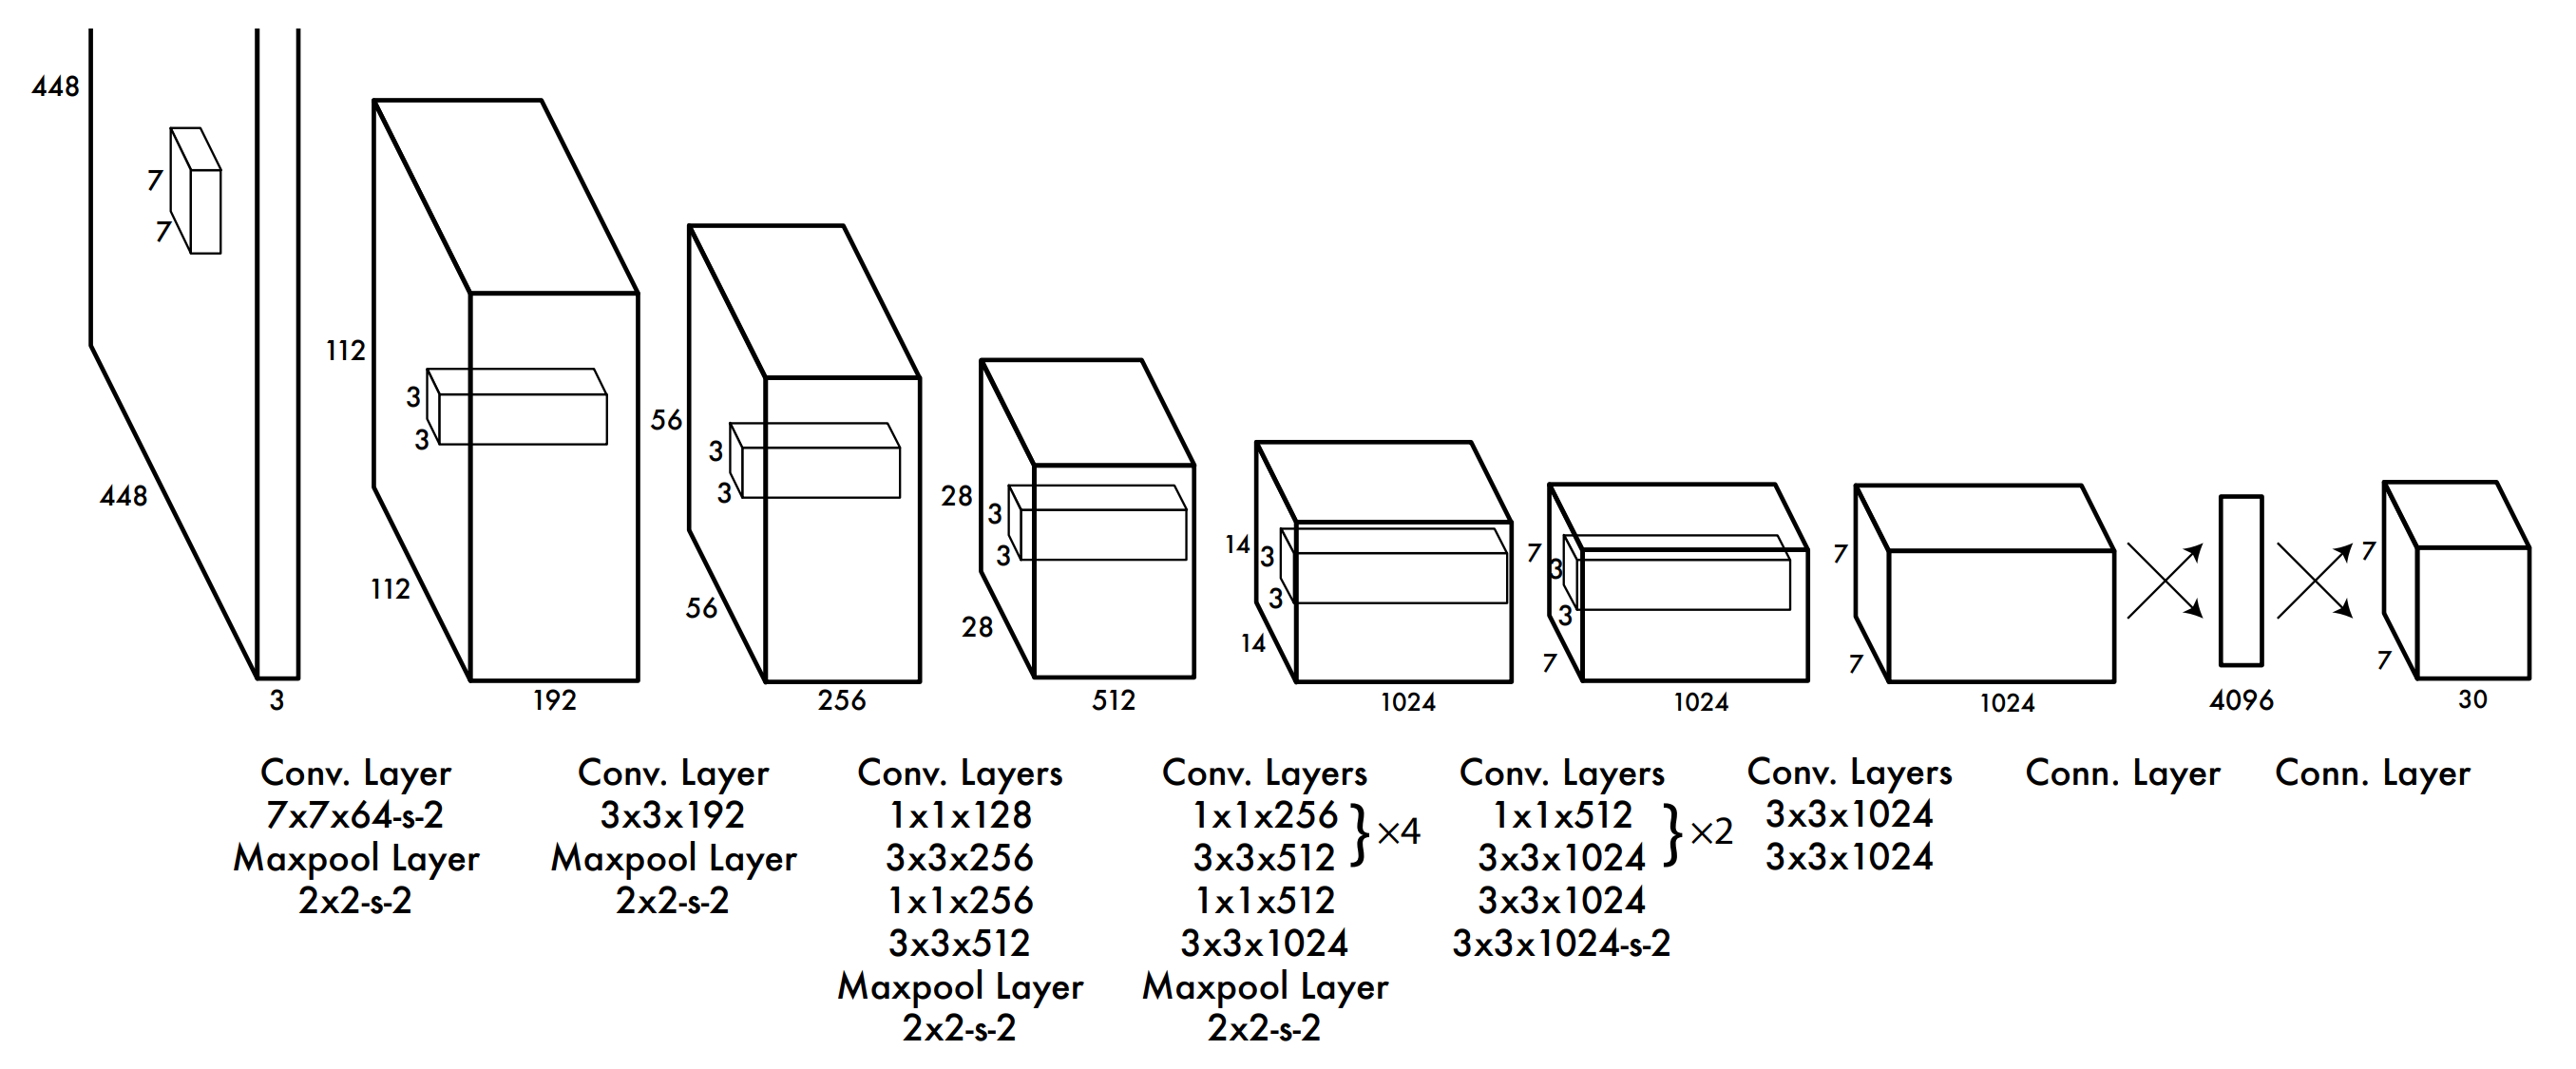
\includegraphics[width = 0.9\textwidth]{yolo框架.png}
    \caption{YOLO算法框架}
    \label{yk}
\end{figure}

(1)对于输入的原图像,在图像中固定地划分出一个 $7 \times 7$ 的网格状区域。

(2)对之前一步中划分出的每个网格,进行检测,每个网格预测出两个bounding box,而每个bounding box中包含目标的位置坐标(x,y,w,h)、置信概率(confidence)、类型信息和相应概率。

(3)在推理后运用非极大值抑制(Non-Maximum Supression)算法,对预测得到的$7 \times 7 \times 2$ 个预测窗口进行筛选,去掉可能性较低的窗口,提高整体的运行效率,从而使得YOLO算法能够达到实时性的要求。

在大幅优化目标检测算法的速度的同时,YOLO算法还存在问题。YOLO 算法主要的局限性在于:

(1)对于输入图像,YOLO算法只能接受尺寸是$448 \times 448$的图像。

(2)由于对每个固定的网格,YOLO算法只能进行两个目标框的预测,对于目标尺寸较小或者某区域内目标较为密集的情况,YOLO算法的定位和检测效果较差。

(3)检测不同大小的 bounding box 在损失函
数中的权重相同。

(4)总的来说,虽然 YOLO算法的模型推理速度很快,能够实现对目标的实时检测,但是YOLO算法的检测精度相比Faster R-CNN 等两阶段目标检测算法仍然较低。

针对上述问题,YOLO系列算法一直在研究如果提高目标检测精度的同时保证算法的推理速度。经过不断的研究和实验,研究人员提出了 YOLOv2\cite{redmon2017yolo9000}、YOLOv3\cite{redmon2018yolov3}和YOLOv4\cite{AlexeyBochkovskiy2020YOLOv4OS}算法。

YOLOv2,又称为YOLO9000,主要特点是提出了一个当时最好的可以实时检测9000种目标类别的系统,因此命名为YOLO9000。在目标检测数据集PASCAL VOC 和 COCO数据集上获得了当时最好的性能。使用多尺度训练的创新方法,YOLOv2模型能够检测不同大小的物体,同时保持了速度和准确率的平衡。在67FPS的速度下,YOLOv2在VOC2007数据集上可以得到了$76.8\%$的准确率。

YOLOv2算法在 YOLO算法 的基础上进行
的改进主要有:

(1)引入了批标准化(Batch Normalization)。批标准化的作用是在大幅提高收敛性能的同时不再需要其他形式的标准化。通过对YOLO模型中所有的卷积层添加了批标准化模块,算法的mAP提高了$2\%$。此外,添加批标准化模块的网络模型中可以不再需要通过dropout层解决拟合问题。

(2)引入高分辨率分类网络,结果是提升了网络输出的 特征图的分辨率,在经过微调后网络的mAP可以提高$4\%$。

(3)YOLOv2不再使用全连接层,而是使用anchor boxes对bounding boxes进行预测。在应用anchor boxes方式后,YOLOv2算法的mAP出现了小幅降低。在应用anchor boxes之前,模型获得了$69.5\%$的mAP和$81\%$的召回率,而在应用anchor boxes之后模型获得了$69.2\%$的mAP和$88\%$的召回率。从该实验结果可以看出,虽然mAP小幅降低,但是召回率的提高意味着模型有很大的改进空间。

(4)维度集群。首先是手工选择anchor box。虽然网络可以自适应地学习
如何适当地调整bounding boxes,但如果选择更好的先验bounding boxes
可以让网络更容易得到更好的检测结果。

(5)引入细粒度特征。在改进的YOLO算法中,网络对
$13\times13$特征图进行检测。虽然这种检测方式在检测大型目标时已经足够,但是在定位较小尺寸的对象时,模型还是需要更细粒度的特征帮助提升性能。Faster R-CNN和SSD算法都选择在各种不同尺寸的特征图上运行他们的区域选择网络,
通过网络获得一系列分辨率的特征。YOLOv2种采用一种不同的细粒度特征提取方法,在网络中简单地添加一个传递层,将早期的
$26\times26$分辨率的特征引入后续的特征图中。

(6)多尺度训练。为了使YOLOv2的算法模型能够鲁棒地运行在各种尺寸的输入图像上,训练过程中引入了各种尺寸的图像,帮助模型更好地学习获取不同尺寸图像的特征。

YOLOv3算法对YOLO系列进行了很大的更新。该算法使用了许多小的设计使得模型获得了更好的性能。在训练了新的网络并进行实验后可以看出,YOLOv3的性能确实大幅超过了YOLO9000。YOLOv3模型比YOLOv2略大,但是准确率更高。与此同时,YOLOv3算法依然很快。在$320\times320$的图片上进行对比实验,YOLOv3算法的推理时间为22ms,准确率为$28.2\%$,这一结果与SSD相近,但是YOLOv3的速度快了3倍。当使用0.5IoU mAP测试标准时,YOLOv3算法获得了$57.9\%$的准确率,推理时间为51ms,而RetinaNet获得了$57.5\%$准确率的同时消耗了198ms,因此YOLOv3大约比RetinaNet快3.8倍。

YOLOv3算法的主要改进是:

(1)将FPN的思想引入YOLOv2网络中。YOLOv3能在3个不同的特征尺度上进行目标检测,对每个网格设置3个先验的anchor box,对每个不同大小的特征图分别预测目标的位置及类型信息。

(2)通过研究residual network将基础网络改进为Darknet-53,该网络相比以往层数更深,特征提取能力更强。

(3)在损失函数方面,采用logistics取代原来的softmax来实现对多标签的分类预测,适应更多类型标签的数据集,获得更好的类型泛化能力。

后续的YOLOv4网络在当时取得了目标检测领域最佳的精度和速度。YOLOv4的主要创新有:

(1)使用了Mish激活函数。经过实验,用Mish激活函数取代Leaky ReLU激活函数后,图像分类任务中的精度都得到了提高。

(2)引入了dropblock方法\cite{ghiasi2018dropblock}来缓解过拟合问题。和传统的dropout方法不同的是,dropout是随机丢弃某些神经元来使网络结构变得简单,而dropblock的处理方法是对某个局部区域进行删减。

在YOLO系列研究人员不断提出更好性能的目标检测算法的同时,另外一个研究提升单阶段目标检测算法性能的一个分支是 SSD 系列, 2016 年 Liu W 等人通过分析借鉴 YOLO 的回归思想,在此基础上融合了 Faster R-CNN 的 anchor 机制,力求将YOLO的快速和Faster R-CNN的精度高这两个特点结合起来,对不同尺度的特征图和不同大小的目标进行检测和将结果进行筛选和合并。从YOLO和SSD各自的网络结构可以看出,SSD算法选择将不同网络层输出的各个特征图都进行目标位置和类型的训练和预测,以此来实现对各种尺寸目标的检测。而YOLO算法中仅仅在最后一层进行目标的训练和检测,而经过网络若干的池化层后,最后一层特征图的尺寸将会大大缩小,对应原图像中的区域就会很大,因此YOLO对小目标的检测能力较弱。SSD和YOLO的这一处理方法的不同,导致SSD对小目标的检测精度明显高于YOLO算法。SSD的算法框架如图\ref{ssd}所示。

\begin{figure}[htbp]
    \centering
    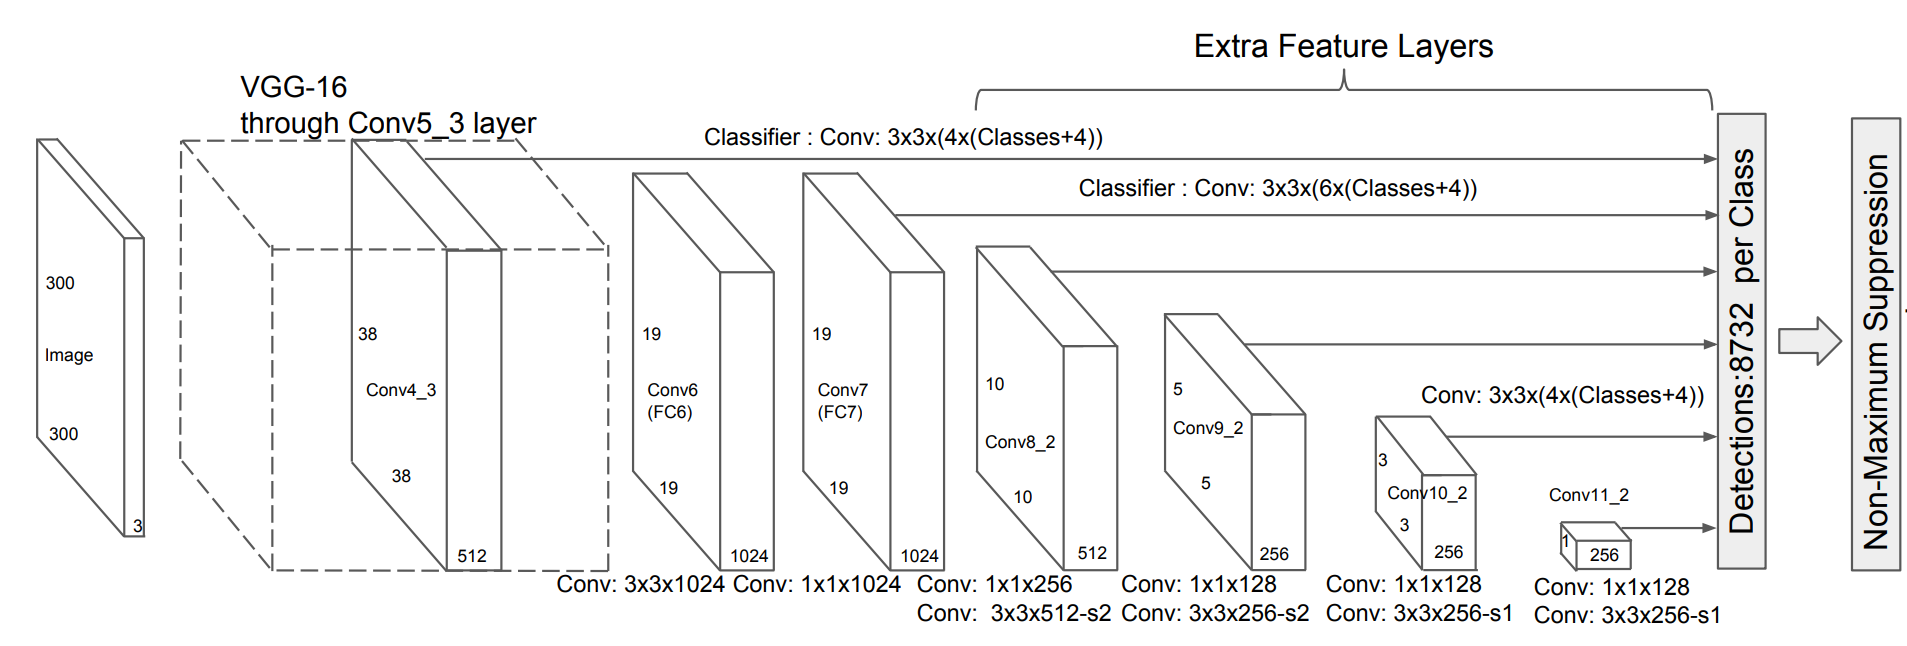
\includegraphics[width = 0.9\textwidth]{ssd.png}
    \caption{SSD算法框架}
    \label{ssd}
\end{figure}

SSD算法的初衷是将YOLO算法和Faster R-CNN算法的优势进行结合,同时获得高速度和高精度。但是SSD算法仍然存在问题,主要的局限性有:

(1)虽然引入了特征金字塔的思想,对不同尺度特征图都进行检测,但是需要人工设置prior box的min size,max size和aspect ratio值。SSD网络中prior box的基础大小和形状都不是直接通过学习获得,而是通过手工进行设置。但是网络中每一层特征图使用的prior box大小和形状都各不相同,因此该算法的调试是一项比较困难的工作。

(2)虽然采用了特征金字塔的思路,但是SSD算法对小目标的召回率表现依然一般,并没有实现大幅领先Faster R-CNN的效果。这是由于SSD使用低级特征提取层去检测小目标,而低级特征卷积层数少,存在特征提取不充分的问题。

在SSD算法提出后,研究人员不断对SSD算法提出改进。
近几年,在SSD算法的基础上,衍生出了很多改进版本,主要有 DSSD\cite{fu2017dssd}、
DSOD\cite{shen2017dsod}和FSSD\cite{li2017fssd}等。

DSSD的主要贡献是在通用目标检测算法中引入附加上下文的方法。为了实现这一点,作者首先将最先进的分类器(Residual-101)与快速检测框架(SSD)相结合,之后用反卷积层来增强SSD+Residual-101,以在目标检测中引入额外的大规模背景,并提高算法的目标检测精度,尤其是小目标的检测精度。因此该系统称为DSSD。结果显示PASCAL VOC和COCO数据集的实验中,使用$513 \times513$输入图像的DSSD在VOC2007测试上获得了$81.5\%$的mAP,在VOC2012数据集上获得了$80.0\%$的mAP,在COCO数据集上获得了$33.2\%$的mAP。实验结果表明,DSSD算法在每个数据集上都超过了当时最好的R-FCN方法。

DSSD 主要研究了SSD算法对小目标的检测能力不够强的问题,作者认为这是SSD网络中的浅层特征图的语义信息较少导致的,据此提出了一种将特征图进行上采样处理后再和原始的特征图进行拼接的方法,来提高模型对不同尺寸特征的表达能力。但是DSSD模型的灵活性不够,耗时较大。

在研究分析了以上问题后,Zhiqiang Shen等人提出了 DSOD 算法。这种算法不再需要是一预训练模型,在目标检测任务中可以实现从零开始进行模型权重的训练,并且效果不弱于微调过的模型。DSOD算法可以看作是 SSD算法和DenseNet 算法的结合,在精度较高的同时减少了参数量。

\subsection{红外图像目标检测研究现状}
最近几年,随着红外成像技术和设施的不断成熟,红外成像的全天候等特性,使得红外目标检测领域受到了越来越多研究人员的关注。与此同时,红外图像相比可见光图像还存在一定的缺陷。红外图像一般对比度较低,成像的目标上纹理信息较少,图像的整体信噪比不高,这些特点使得红外图像的目标检测任务难度更大。因此红外目标检测算法未来的主要研究方向就是如何针对红外图像中的主要问题进行优化,从而提高红外目标检测算法的性能,使得红外目标检测应用范围更广,帮助更多领域更好地执行检测任务。

目前的红外图像目标检测算法,存在几种不同的研究方向。目前主要可以将红外图像目标检测算法分成以下几种类别:基于目标的先验知识的检测算法、使用模板匹配的检测算法、基于机器学习的检测算法等。

在待测目标和背景之间的对比度较高时,往往可以利用目标的先验知识对红外图像中的目标进行检测,这种情况中场景简单,但是往往需要手动简历一个数据库用于存放先验知识,将目标提取的特征和数据库进行比对后判定目标是否为待测的某个类型。这种算法的实现较为复杂,而且泛化能力不足,一旦检测的目标或是环境发生变化,该算法的先验知识和数据库就要重新开始建立。因此该方法的灵活性较差,不能适应大多数的红外图像目标检测场景。

在之后的研究中,有研究人员提出根据统计方法从数据中提取出模板,将红外图像和模板直接进行匹配后得到目标的位置和类型信息\cite{宋曦2010一种基于模板匹配的目标识别方法}。针对模板匹配的精度问题,可以针对不同的场景对模板进行独立的设计和生成,通过验证,人工设计的模板可以提升红外图像目标检测的精度。

1997 年,Maes 等人提出了一种用于多模图像配准的定量-定性互信息度量\cite{maes1997multimodality}(Q-MI)方法。传统的信息度量方法如香农熵和互信息存在的问题是,只反映了信息的定量方面而忽略了信息的定性方面,因为传统方法往往只研究事件的概率。而实际上每个事件都对实现潜在目标产生了各自的影响,这种影响往往独立于其发生的概率。因此,这种互信息度量方法中重点考虑信息的定量和定性的整体衡量标准,以实现对事件特征信息的更合适的度量。由于具有较高效用值的因素在测量两幅图像的Q-MI方面贡献更大,因此基于Q-MI的配准方法比传统的基于MI的配准方法具有更强的鲁棒性。此外,基于Q-MI的配准方法可以提供更平滑的配准功能,捕获范围也相对更大。该算法提出的Q-MI方法已被应用于医学临床的MR、CT和PET图像的配准任务中。
1999 年,Studholme C 等人研究了重叠统计量等问题\cite{studholme1999overlap},提出了用梯度指标来解决联合熵的问题,在此基础上将互信息进行归一化等处理,解决了互信息不能提供有用的对齐措施的问题。通过实验结果可知,该方法可以实现对目标的快速检测。
之后,Russakoff 等人研究并发现,将互信息用来作为图像中的相似程度的指标的方式缺少空间相关性,因此提出将空间信息添加到互信息中,提出了基于区域互信息的图像相似性度量方法\cite{russakoff2004image}。
2005 年,顾静
良等人研究了红外弱小目标的检测识别问题,提出了一种针对性的相似性度量方法,主要解决的问题是在红外图像中的大量噪声和弱小目标等条件下进行目标的检测和识别,并且在此基础上对模板匹配方法进行了改进,应用自适应模板匹配方法提高了算法的稳定性和鲁棒性\cite{顾静良2005基于自适应模板匹配的红外弱小目标检测}。
2008 年,钟都都等人研究了红外图像目标检测的实时性和抗漂移问题\cite{钟都都2008用于红外目标跟踪的模板匹配改进算法},提出了一种目标跟踪算法,将算法的模板匹配方法进行了改进,提出用SUSAN算子对目标的特征角点,将特征信息和灰度信息通过加权合并的方式获得模板。实验证明该算法可以在保证实时性的基础上获得一定的稳定性。虽然模板匹配相对于先验匹配实现简单,但是模板的选择和改进仍然需要大量的工作,该方法的适用范围仍然较小,常常应用于较简单的红外图像目标检测场景。

基于机器学习的红外目标检测方法主要可以分为两类:一类是传统的机器学习算法,通过对特征进行手工提取后,输入分类器中进行分类。另一类是用深度神经网络进行红外目标的定位和分类。
传统机器学习方法主要可以分
为三个步骤,分别是区域选择、特征提取和分类。
之后的研究中,还有研究人员提出基于目标特性进行 ROIs
区域搜索和阈值分割等方法。

在深度学习算法和深度学习配套的计算设施出现之前,基于机器学习的红外目标
检测算法因其较强的鲁棒性和相对较好的性能,成为红外目标检测领域的主流算法。但是传统机器学习算法存在大量的计算开销,并且因为红外图像本身存在大量的噪声、信噪比低等问题,传统机器学习算法在红外图像目标检测任务的效果弱于基于深度学习的算法。
近几年随着深度学习算法和硬件计算能力的发展,卷积神经网络的数据处理和特征表达能力越来越强大,在可见光目标检测领域已经表现出了很强的性能。研究人员也在不断研究红外图像中的深度学习目标检测算法。
Aparna
Akula 等人通过自建红外
数据集,开发除了一种隐私保护系统,主要功能是识别人的行为。主要工作是针对数据集设计了一种目标检测网络,实验数据表明,检测精度可以达到 $87.44\%$。该算法的提出验证了卷积
神经网络用于红外目标检测的可行性\cite{akula2018deep}。
许来祥等人提出了一种基于 ZFNet 改进的目标检测网络,该改进方法主要特点是结合红外图像的各种特点,在 ZFNet 基础上通过增加一种空间变换网络来提高算法的
鲁棒性。不仅如此,该算法深入研究了 Dropout 层各种不同参数的设置对整个检测系统性能的影响\cite{许来祥2020基于改进}。目前基于深度
学习的红外图像目标检测的研究较少,主要是开源的红外数据集较少,相信随着更多红外目标数据集的公开,会有更多的研究人员参与红外图像目标检测的相关研究工作。

\section{本文主要研究内容}
本文主要针对红外图像无人机目标检测任务存在的问题进行研究,在课题研究过程中,主要分析并研究了以下几个方面的问题:

(1)红外无人机数据匮乏

目前开源的红外数据比较少,而基于深度学习的目标检测网络需要有充足的
数据支撑,因此本文的研究内容包括了红外无人机目标数据集的标注和制作。

(2)红外图像的检测特点和难点

由于红外图像在获取的过程中主要受到红外探测器和环境噪声的影响以及
红外辐射原理所造成的红外图像质量差、信噪比低等不利于检测的缺点。因此在
网络输入图像之前对红外图像进行预处理提高图像信噪比、增大图像包含的信息量也是重点研究的内容。

(3)待测无人机目标的尺度变化

本文的任务是红外图像无人机目标检测,场景的特点是小目标的出现频率较高,因此算法对较小尺寸目标的检测能力也是本文的研究内容。

(4)无人机目标检测的定位问题

在 YOLOv5 中使用IoU作为损失函数,有可能产生定位不准的问题,因此本文重点研究了对YOLOv5网络目标框定位损失函数的改进。

(5)检测算法的嵌入式实现以及实时推理

在某些特殊应用场景中难以满足较高的计算能力,如在嵌入式设备上使用,
无法保证在速度较快的情况下实现高精度检测,这种时候就需要设计出适用于特
定任务下的轻量级实时目标检测网络,也是本课题重点研究的问题。

\section{本文组织结构}
本文以红外目标检测算法所存在的问题展开研究,研究了红外无人机检测并实现嵌入式应用。本文分为四个章节,每
个章节的主要内容如下:

第1章为绪论。首先介绍了基于深度学习的红外目标检测算法的研究背景和
意义,然后针对当前主流的目标检测算法的国内外研究发展现状做了发展脉络介
绍,介绍了红外目标检测算法在传统方向和深度学习方向的相关研究工作,最后
介绍了本文具体的研究内容和组织结构。

第2章介绍了红外目标检测相关理论和工作基础。首先介绍了卷积神经网络
的主要组成结构以及目标检测的评价指标,接着对红外图像如何获得的过程进行
了简单的介绍,最后介绍了红外图像的主要特征。

第3章主要介绍了建立红外无人机图像数据集的过程,研究了目前主流的图像预处理方法,并进行了测试,用以提高整
个图像的信息量,并提出了两种新的红外数据增强算法,并将该算法在数据集上
进行了测试和结果分析,此外还对YOLOv5网络的目标框定位损失函数进行了改进,并对改进后的算法进行了实验和分析。

第4章实现红外无人机检测的轻量化和实时嵌入式应用。由于实际项目需要完成对无
人机的实时检测,因此本文重点研究了算法的轻量化和嵌入式部署,将第三章中研究的较高精度的红外无人机检测算法通过轻量化方法实现精度和速度的平衡,然后将得到的新算法部署在嵌入式设备上,进行更加贴近红外无人机检测应用场景的功能测试,基本可以达到实时推理,验证本文研究算法的适用性。


